\documentclass[12pt,a4paper]{article}
\usepackage[brazilian]{babel}
\usepackage[utf8]{inputenc}
\usepackage[T1]{fontenc}
\usepackage{amsmath,amssymb}
\usepackage{graphicx}
\usepackage{hyperref}
\usepackage{xurl}
\usepackage{geometry}
\geometry{margin=2.5cm}

\title{Prova 01 - Resolucao das Questoes (a partir das imagens)}
\author{Disciplina: Principios de Modelagem Matematica e Computacional}
\date{14/04/2026}

\begin{document}
\maketitle

\section*{Questao 1 - Dimensao fractal dos conjuntos}
Pelas figuras da prova, os dois conjuntos correspondem a:
\begin{itemize}
  \item curva do tipo Koch (auto-similar com $N=4$ copias e fator de escala $r=1/3$);
  \item conjunto triangular auto-similar com $N=4$ e $r=1/2$.
\end{itemize}

Para conjuntos auto-similares, a dimensao fractal e:
\begin{equation}
D = \frac{\ln N}{\ln(1/r)}.
\end{equation}

\textbf{(1) Curva tipo Koch:}
\begin{equation}
D_1 = \frac{\ln 4}{\ln 3} \approx 1.2619.
\end{equation}

\textbf{(2) Conjunto triangular da figura:}
\begin{equation}
D_2 = \frac{\ln 4}{\ln 2} = 2.
\end{equation}

\subsection*{Figura de apoio (internet)}
\begin{figure}[htbp]
\centering
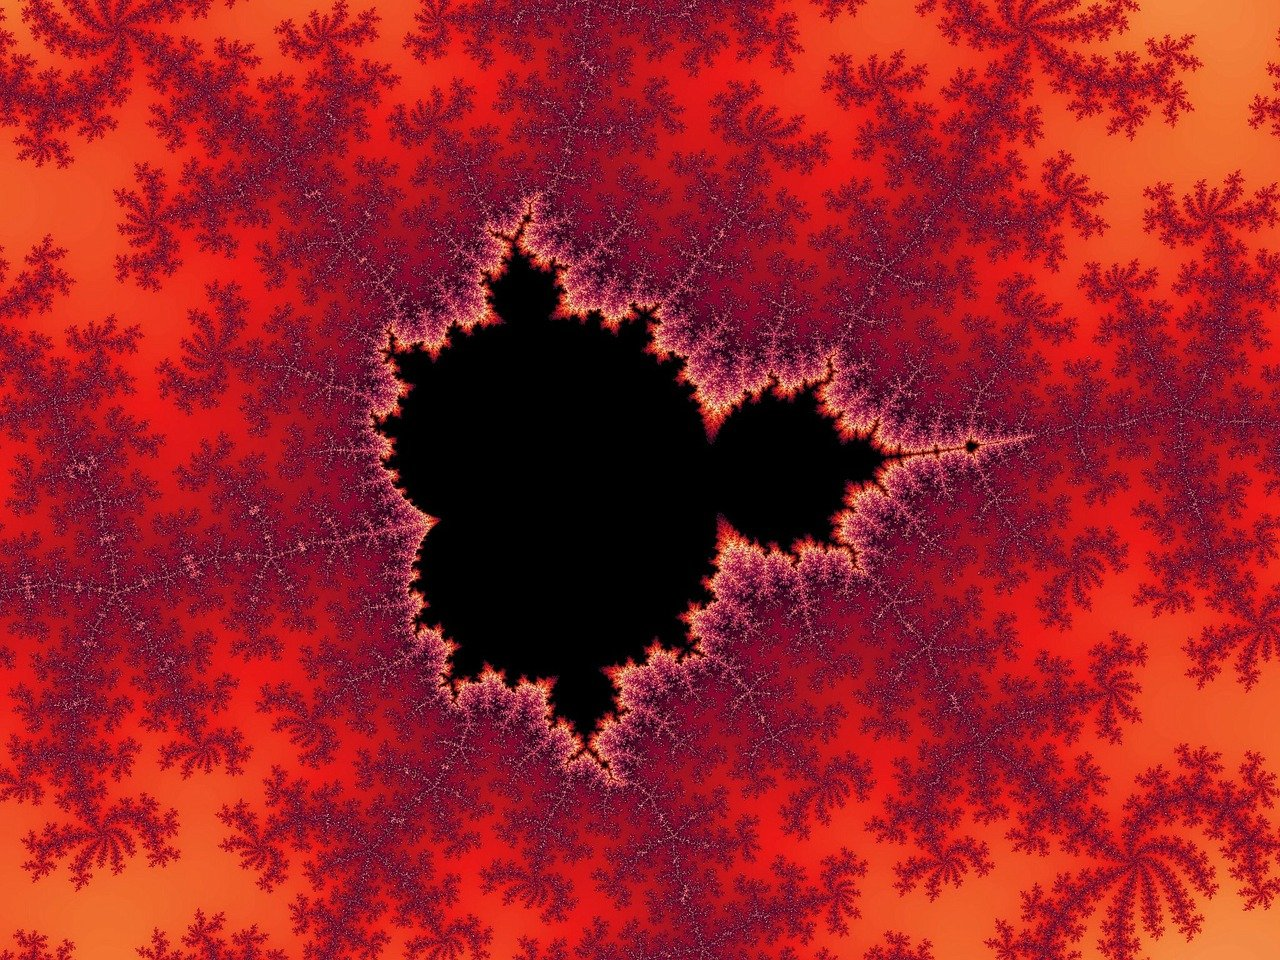
\includegraphics[width=0.55\textwidth]{figuras_web/fractal_mandelbrot.jpg}
\caption{Fractal de Mandelbrot (apoio visual para a Questao 1).}
\end{figure}
Fonte: \url{https://commons.wikimedia.org/wiki/Special:FilePath/Mandelbrot-293453_1280.jpg}

\section*{Questao 2 - Relacao para a frequencia de oscilacao}
Enunciado (resumo): uma viga de massa $m$ e cabo de comprimento $L$, sob gravidade $g$ e tensao $\tau$, oscila com frequencia $\omega$. Pedem uma relacao para estimar $\omega$ em funcao da altura $h$.

\subsection*{Passo 1: Variaveis do problema}
\begin{equation}
\omega,\; h,\; m,\; g,\; \tau,\; L.
\end{equation}

\subsection*{Passo 2: Dimensoes fundamentais}
\begin{equation}
[\omega]=T^{-1}, \quad [h]=L, \quad [L]=L, \quad [m]=M, \quad [g]=LT^{-2}, \quad [\tau]=MLT^{-2}.
\end{equation}

\subsection*{Passo 3: Numero de grupos adimensionais}
Temos $n=6$ variaveis e $k=3$ dimensoes fundamentais ($M,L,T$). Pelo Teorema de Buckingham:
\begin{equation}
n-k=6-3=3.
\end{equation}
Logo, precisamos de 3 grupos adimensionais.

\subsection*{Como escolher as variaveis adimensionais (regra pratica)}
Para montar os grupos $\Pi$ sem erro, siga este roteiro curto:
\begin{enumerate}
  \item Escolha $k$ \textbf{variaveis repetidas} (aqui, $k=3$): elas devem ser dimensionalmente independentes e, juntas, conter $M$, $L$ e $T$.
  \item Evite colocar a variavel dependente ($\omega$) no conjunto repetido, para facilitar o isolamento final de $\omega$.
  \item Cada variavel restante gera um grupo $\Pi$: escreva essa variavel multiplicada pelas repetidas elevadas a expoentes desconhecidos.
  \item Impoe adimensionalidade: zere os expoentes de $M$, $L$ e $T$ para resolver o sistema linear.
  \item Se aparecerem grupos diferentes dos de outro colega/livro, tudo bem: bases diferentes sao equivalentes se forem combinacoes adimensionais entre si.
\end{enumerate}

Neste problema, uma escolha boa de repetidas e $m,\,g,\,h$, porque:
\begin{equation}
[m]=M,\qquad [g]=LT^{-2},\qquad [h]=L,
\end{equation}
ou seja, cobrem $M,L,T$ e sao independentes.

\subsection*{Passo 4: Escolha dos grupos $\Pi$}
Escolhemos como variaveis repetidas $m,\,g,\,h$ (independentes e cobrindo $M,L,T$).

\textbf{Grupo envolvendo $L$:}
\begin{equation}
\Pi_1 = L\,m^{a}g^{b}h^{c}.
\end{equation}
Dimensoes:
\begin{equation}
[\Pi_1]=L\cdot M^{a}(LT^{-2})^{b}L^{c}=M^aL^{1+b+c}T^{-2b}.
\end{equation}
Para ser adimensional, os expoentes de $M,L,T$ devem ser zero:
\begin{equation}
a=0,\qquad -2b=0\Rightarrow b=0,\qquad 1+b+c=0\Rightarrow c=-1.
\end{equation}
Logo:
\begin{equation}
\Pi_1=\frac{L}{h}.
\end{equation}

\textbf{Grupo envolvendo $\omega$:}
\begin{equation}
\Pi_2 = \omega\,m^{a}g^{b}h^{c}.
\end{equation}
Dimensoes:
\begin{equation}
[\Pi_2]=T^{-1}\cdot M^{a}(LT^{-2})^{b}L^{c}=M^aL^{b+c}T^{-1-2b}.
\end{equation}
Sistema:
\begin{equation}
a=0,\qquad -1-2b=0\Rightarrow b=-\frac12,\qquad b+c=0\Rightarrow c=\frac12.
\end{equation}
Assim:
\begin{equation}
\Pi_2=\omega\sqrt{\frac{h}{g}}.
\end{equation}
Forma equivalente (inversa ao quadrado), usada na conta final:
\begin{equation}
\Pi_2' = \frac{g}{h\omega^2}.
\end{equation}

\textbf{Grupo envolvendo $\tau$:}
\begin{equation}
\Pi_3 = \tau\,m^{a}g^{b}h^{c}.
\end{equation}
Com $[\tau]=MLT^{-2}$:
\begin{equation}
[\Pi_3]=MLT^{-2}\cdot M^{a}(LT^{-2})^{b}L^{c}
=M^{1+a}L^{1+b+c}T^{-2-2b}.
\end{equation}
Sistema:
\begin{equation}
1+a=0\Rightarrow a=-1,
\qquad
-2-2b=0\Rightarrow b=-1,
\qquad
1+b+c=0\Rightarrow c=0.
\end{equation}
Logo:
\begin{equation}
\Pi_3=\frac{\tau}{mg}.
\end{equation}

Portanto, uma base conveniente de grupos adimensionais e:
\begin{equation}
\Pi_1 = \frac{L}{h},
\qquad
\Pi_2' = \frac{g}{h\omega^2},
\qquad
\Pi_3 = \frac{\tau}{mg}.
\end{equation}

Observacao: o expoente extra ($d$) aparece quando se escolhe montar um grupo misturando duas variaveis nao repetidas no mesmo $\Pi$ (por exemplo, $\tau$ e $\omega$). Isso cria uma familia equivalente de grupos, com um grau de liberdade. Para a construcao canonica de Buckingham, cada variavel nao repetida gera um grupo com expoentes apenas nas repetidas.

\subsection*{Como verificar se duas bases de grupos sao equivalentes}
Suponha que outro colega use a base:
\begin{equation}
\widetilde{\Pi}_1=\frac{L}{h},
\qquad
\widetilde{\Pi}_2=\omega\sqrt{\frac{h}{g}},
\qquad
\widetilde{\Pi}_3=\frac{\tau}{mg}.
\end{equation}

Para verificar equivalencia, basta escrever uma base em funcao da outra por combinacoes adimensionais:
\begin{equation}
\Pi_1=\widetilde{\Pi}_1,
\qquad
\Pi_2'=(\widetilde{\Pi}_2)^{-2},
\qquad
\Pi_3=\widetilde{\Pi}_3.
\end{equation}

Como cada grupo de uma base foi escrito como produto/potencia de grupos da outra (e a volta tambem e possivel), as duas bases sao equivalentes.

\textbf{Regra pratica:} se voce consegue transformar uma base na outra usando apenas produto, quociente e potencia entre grupos adimensionais, entao ambas descrevem a mesma fisica e estao corretas.

\subsection*{Passo 5: Relacao funcional e isolacao de $\omega$}
A forma geral e:
\begin{equation}
F(\Pi_1,\Pi_2,\Pi_3)=0.
\end{equation}

Da definicao de $\Pi_2$:
\begin{equation}
\omega \propto \sqrt{\frac{g}{h}}.
\end{equation}

Portanto, uma forma adimensional consistente para a resposta final e:
\begin{equation}
\omega = \sqrt{\frac{g}{h}}\;\Phi\!\left(\frac{L}{h},\frac{\tau}{mg}\right),
\end{equation}
onde $\Phi$ e funcao adimensional.

\begin{figure}[htbp]
\centering
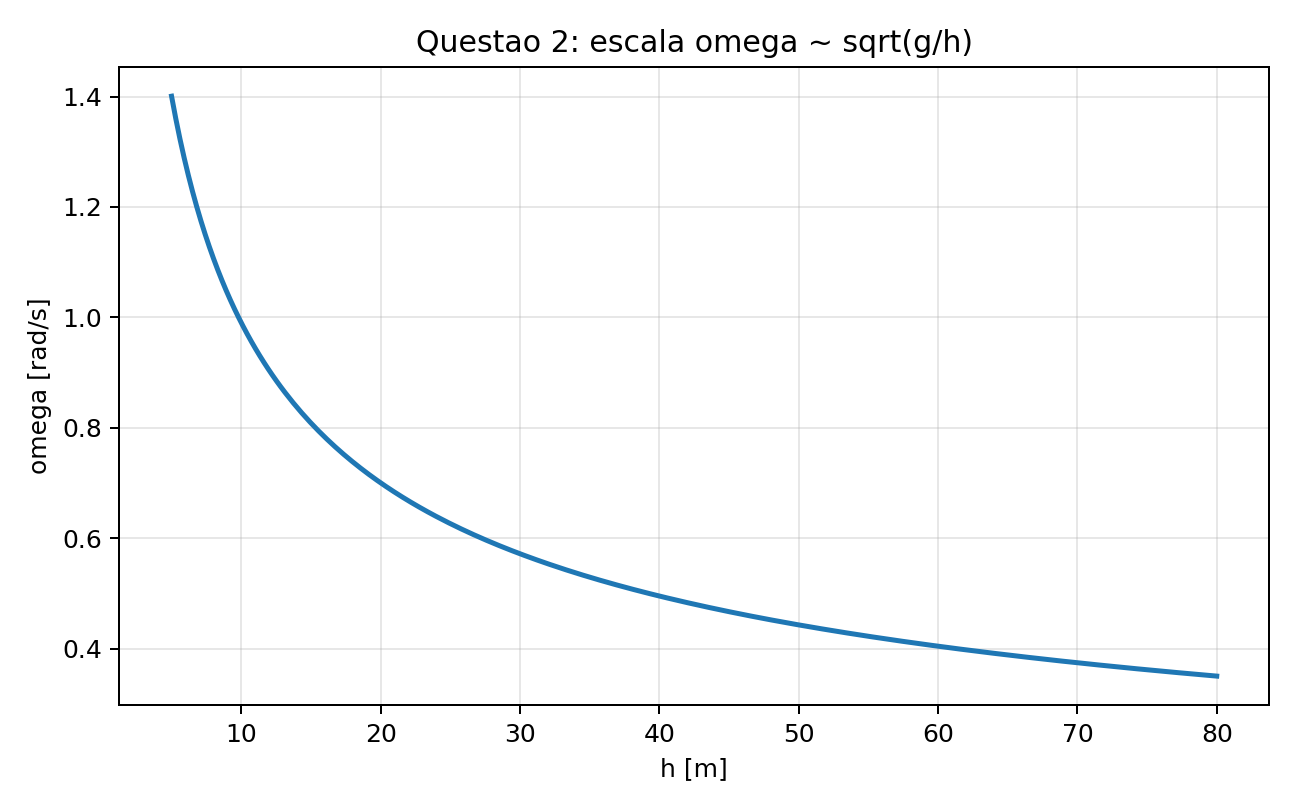
\includegraphics[width=0.75\textwidth]{figuras_prova/q2_escala_omega_h.png}
\caption{Grafico da escala de frequencia para a Questao 2: $\omega\sim\sqrt{g/h}$.}
\end{figure}

\section*{Questao 3 - Depreciacao do carro}
Dados: valor inicial $V_0=\text{R\$ }51.500$ e perda de $12\%$ ao ano.

\subsection*{(a) Funcao do valor apos $t$ anos}
\begin{equation}
V(t)=51500\,(1-0.12)^t = 51500\,(0.88)^t.
\end{equation}

\subsection*{(b) Taxa mensal aproximada}
Se a taxa mensal de depreciacao e $i_m$, entao:
\begin{equation}
(1-i_m)^{12}=0.88.
\end{equation}
Logo:
\begin{equation}
i_m = 1-0.88^{1/12} \approx 0.010596 \approx 1.06\%\text{ ao mes}.
\end{equation}

\subsection*{(c) Grafico da funcao}
A curva de $V(t)=51500\,0.88^t$ e exponencial decrescente, com $V(0)=51500$ e assintota horizontal em $V=0$.

\begin{figure}[htbp]
\centering
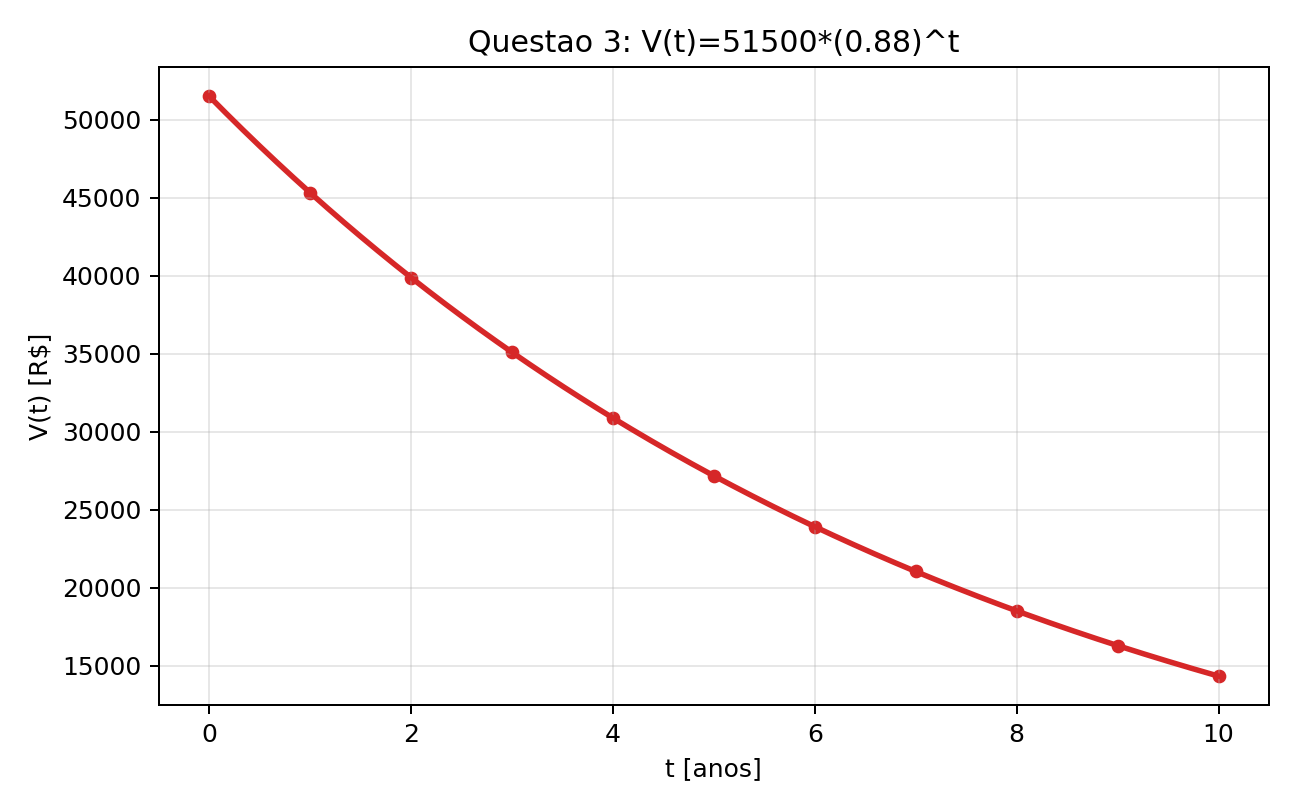
\includegraphics[width=0.75\textwidth]{figuras_prova/q3_depreciacao.png}
\caption{Grafico da funcao de depreciacao da Questao 3.}
\end{figure}

\subsection*{Figura de apoio (internet)}
\begin{figure}[htbp]
\centering
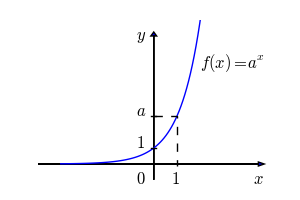
\includegraphics[width=0.55\textwidth]{figuras_web/funcao_exponencial.png}
\caption{Exemplo de grafico de funcao exponencial (apoio para a Questao 3).}
\end{figure}
Fonte: \url{https://commons.wikimedia.org/wiki/Special:FilePath/Exponential_function_defn.png}

\subsection*{(d) Estimativa do valor apos 6 anos}
\begin{equation}
V(6)=51500\,(0.88)^6 \approx \text{R\$ }23.916{,}81.
\end{equation}

\section*{Questao 4 - Gerador linear congruencial}
Gerador:
\begin{equation}
X_{n+1}=(aX_n+c)\;\text{mod}\;m,
\qquad m=10.
\end{equation}

Condicoes para periodo maximo $m$ (Hull-Dobell):
\begin{enumerate}
  \item $\gcd(c,m)=1$;
  \item $a-1$ divisivel por todos os fatores primos de $m$;
  \item se $m$ e multiplo de 4, entao $a-1$ multiplo de 4.
\end{enumerate}

Para $m=10=2\cdot 5$:
\begin{itemize}
  \item escolha $c=9$ (coprimo com 10);
  \item escolha $a=11$ (assim $a-1=10$, divisivel por 2 e 5).
\end{itemize}

Observacao: o par escrito na folha ($a=31$, $c=9$) tambem e valido, pois $31\equiv 1\pmod{10}$ e satisfaz as mesmas condicoes de periodo maximo para $m=10$.

Portanto, um par valido e:
\begin{equation}
(a,c)=(11,9).
\end{equation}

Com isso, o gerador fica:
\begin{equation}
X_{n+1}=(11X_n+9)\;\text{mod}\;10.
\end{equation}
Como $11\equiv 1\;(\text{mod }10)$, isso equivale a:
\begin{equation}
X_{n+1}=(X_n+9)\;\text{mod}\;10,
\end{equation}
que percorre todos os 10 residuos antes de repetir.

\subsection*{Verificacao com 3 sementes}
\textbf{Semente $X_0=0$:}
\begin{equation}
0,9,8,7,6,5,4,3,2,1,0\;(\text{periodo }10).
\end{equation}

\textbf{Semente $X_0=3$:}
\begin{equation}
3,2,1,0,9,8,7,6,5,4,3\;(\text{periodo }10).
\end{equation}

\textbf{Semente $X_0=7$:}
\begin{equation}
7,6,5,4,3,2,1,0,9,8,7\;(\text{periodo }10).
\end{equation}

Logo, a propriedade de periodo maximo foi demonstrada.

\begin{figure}[htbp]
\centering
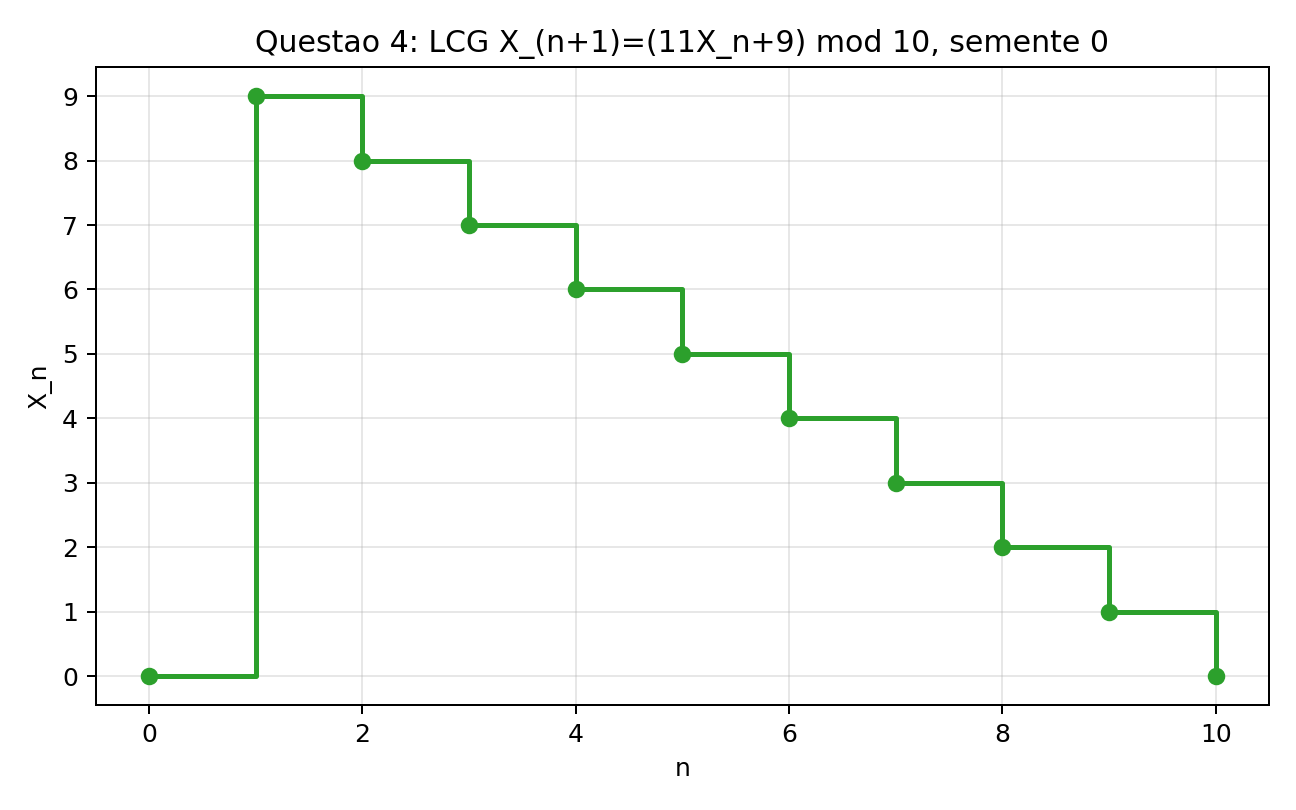
\includegraphics[width=0.75\textwidth]{figuras_prova/q4_lcg_semente0.png}
\caption{Evolucao da sequencia do LCG para semente $X_0=0$ na Questao 4.}
\end{figure}

Referencia de apoio visual/teorica para LCG:
\url{https://en.wikipedia.org/wiki/Linear_congruential_generator}

\section*{Exercicios semelhantes encontrados na internet (para reforco)}
Os problemas abaixo sao do mesmo tipo das questoes da prova e servem para checagem de metodo:

\begin{itemize}
  \item \textbf{Fractais e dimensao:} explicacoes e exemplos de auto-similaridade (inclui Koch e Sierpinski) em
  \url{https://pt.wikipedia.org/wiki/Dimens%C3%A3o_fractal}.

  \item \textbf{Buckingham $\Pi$:} roteiro de 6 passos para montar grupos adimensionais em
  \url{https://pt.wikipedia.org/wiki/Teorema_%CF%80_de_Vaschy-Buckingham}.

  \item \textbf{Funcao exponencial (aplicacoes e exercicios resolvidos):}
  \url{https://mundoeducacao.uol.com.br/matematica/funcao-exponencial.htm}.

  \item \textbf{Grafico exponencial e leitura de comportamento:}
  \url{https://mundoeducacao.uol.com.br/matematica/grafico-funcao-exponencial.htm}.

  \item \textbf{Gerador congruencial linear (periodo e condicoes Hull-Dobell):}
  \url{https://en.wikipedia.org/wiki/Linear_congruential_generator}.
\end{itemize}

\subsection*{Como isso melhora a resolucao desta prova}
\begin{enumerate}
  \item Confirma a formula de dimensao fractal usada na Questao 1.
  \item Valida a estrategia de grupos adimensionais da Questao 2.
  \item Confere o raciocinio de depreciacao exponencial da Questao 3 com exercicios equivalentes.
  \item Reforca formalmente as condicoes de periodo maximo do LCG da Questao 4.
\end{enumerate}

\end{document}
